%!TEX root = ../Fast_Contour_Tracing_Algorithm.tex
% -*- root: ../Fast_Contour_Tracing_Algorithm.tex -*-

\section{Related Works}

% Most conventional contour tracing algorithms run on two-dimensional (2D) binary images that consist of black-and-white pixels, which are obtained through binarization, for determining whether a pixel has dark or light intensity. In the digitized image, we can assume that the objects have black pixels and the background has white pixels; therefore, a contour pixel is black and it has at least one adjacent pixel that is white.

To determine whether a pixel has a dark or light intensity, most conventional contour-tracing algorithms are used to process two-dimensional (2D) binary images that consist of black-and-white pixels that are obtained through binarization. In the digitized image, we can assume that the objects have black pixels and the background has white pixels; therefore, a contour pixel is black and it has at least one adjacent pixel that is white.

\subsection{Overview}

%%% Image 1
\begin{figure}[htbp]
	\centering
	\subfloat[]{ 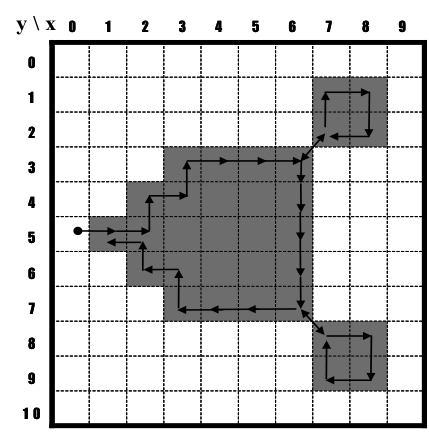
\includegraphics[width=0.3\textwidth, height=5cm]{2.RelatedWorks/fig1-a.png} \label{fig:img1-a} }
	\subfloat[]{ 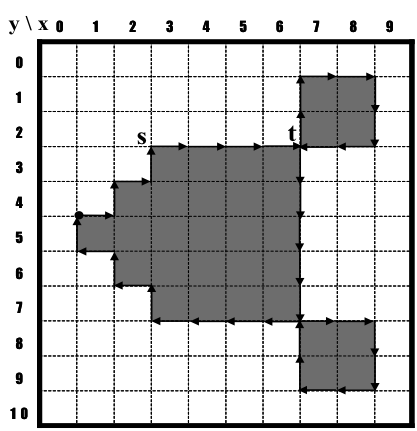
\includegraphics[width=0.3\textwidth, height=5cm]{2.RelatedWorks/fig1-b.png} \label{fig:img1-b} }
	\subfloat[]{ 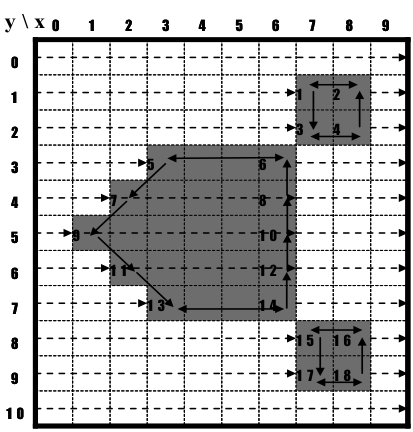
\includegraphics[width=0.3\textwidth, height=5cm]{2.RelatedWorks/fig1-c.png} \label{fig:img1-c} }
	 
	\caption{Contour tracer. \protect\subref{fig:img1-a} Pixel following algorithm \protect\subref{fig:img1-b} Vertex following algorithm \protect\subref{fig:img1-c} Run-data-based following algorithm}
	\label{fig:image1}
\end{figure}

% Figure \ref{fig:image1} shows examples of contour traces obtained by using the contour tracing algorithms. The conventional contour algorithms can be categorized typically into three types as follows: pixel following, vertex following, and run-data-based following \cite{Miyatake1997Contour,Danielsson1981Improvement,Shoji1999Contour}. Among these, the pixel following method is most the common.

Figure \ref{fig:image1} shows examples of contour traces that were obtained using the contour-tracing algorithms. The conventional contour algorithms can typically be categorized into three types as follows: pixel following, vertex following, and run-data-based following \cite{Miyatake1997Contour,Danielsson1981Improvement,Shoji1999Contour}. Of these, the pixel-following method is the most common.

\subsubsection{Pixel-following Method}

% The pixel following method traces contour pixels in a predefined manner and then saves their coordinates in the memory according to the trace order. In figure \ref{fig:img1-a}, the algorithm traces contour pixels along the clockwise direction from the current pixel, i.e., it sequentially searches adjacent black pixels of the current pixel using a relative directional order such as left, front-left, front, front-right, right, right-rear, and rear. Pixel following methods such as simple boundary follower (SBF) \cite{Pitas2000Digital,Das1990Bivariate,Papert1973Uses}, modified SBF (MSBF)\cite{Gose1996Pattern}, improved SBF (ISBF)\cite{Cheong2006Improved}, Moore-Neighbor tracing (MNT) \cite{Toussaint????Grids}, modified MNT (MMNT) \cite{Pradhan2010Contour}, radial sweep algorithm (RSA) \cite{Mirante1982Radial}, and Theo Pavlidis algorithm (TPA)\cite{Pavlidis2012Algorithms} have simple rules for tracing contour pixels based on a chain code. On the contrary, this method requires frame size memory to trace the contour, and it also generates erroneous images when the contour image is enlarged\cite{Miyatake1997Contour} since it maintains only the pixel coordinates.

The pixel-following method traces contour pixels in a predefined manner, and then saves their coordinates in memory according to the trace order. In Figure \ref{fig:img1-a}, the algorithm traces contour pixels along the clockwise direction from the current pixel, i.e., it sequentially searches adjacent black pixels of the current pixel using a relative directional order such as left, front-left, front, front-right, right, rear-right, and rear. Pixel-following methods such as the simple boundary follower (SBF) \cite{Pitas2000Digital,Das1990Bivariate,Papert1973Uses}, modified SBF (MSBF) \cite{Gose1996Pattern}, improved SBF (ISBF) \cite{Cheong2006Improved}, Moore-Neighbor tracing (MNT) \cite{Toussaint????Grids}, modified MNT (MMNT) \cite{Pradhan2010Contour}, radial sweep algorithm (RSA) \cite{Mirante1982Radial}, and Theo Pavlidis algorithm (TPA) \cite{Pavlidis2012Algorithms} have simple rules for tracing contour pixels based on a chain code. On the contrary, this method requires a frame-size memory to trace the contour, and it generates erroneous images when the contour image is enlarged \cite{Miyatake1997Contour} because it maintains only the pixel coordinates.

\subsubsection{Vertex-following Method}
% The vertex following method traces the vertices of the contour pixels that are located on the edges between the contour pixels and the background pixels \cite{Miyatake1997Contour}. Its procedure is similar to that of the pixel following method since it uses a chain code and requires a frame size memory for contour tracing; however, it traces the corners of the contour pixels and their connected edges. Moreover, it stores the corner points of the contour pixels in order to save the traced contour information and the data can be compressed by reducing the number of points in a straight line. For example, in figure \ref{fig:img1-b}, five points of the contour from s to t can be stored as just two points such as (2.5, 2.5) and (6.5, 2.5) based on the (x, y) coordinate system. Moreover, when the contour images are enlarged, the vertex following method can provide the correct image \cite{Miyatake1997Contour} since the traced points form the boundaries of the contour.

The vertex-following method traces the vertices of the contour pixels that are located on the edges between the contour pixels and the background pixels \cite{Miyatake1997Contour}. Its procedure is similar to that of the pixel-following method because it uses a chain code and requires a frame-size memory for contour tracing; however, it traces the corners of the contour pixels and their connected edges. Moreover, it stores the corner points of the contour pixels in order to save the traced contour information, and the data can be compressed by reducing the number of points in a straight line. For example, in Figure \ref{fig:img1-b}, five points of the contour from s to t can be stored as there are only two corner points, i.e., $(2.5, 2.5)$ and $(6.5, 2.5)$ based on the $(x, y)$ coordinate system. Moreover, when the contour images are enlarged, the vertex-following method can provide the correct image \cite{Miyatake1997Contour} because the traced points form the boundaries of the contour.

\subsubsection{Run-data-based Following Method}
% The run-data-based following method, involving the edge-point tracing of rundata \cite{Miyatake1997Contour,Shoji1999Contour},  uses run data in pairs consisting of the left and right edges of an object obtained by horizontal scan lines from left to right on an image. The object can have an outer contour and additional inner contours; therefore, the run data has five types: (left edge of outer contour, right edge of outer contour), (left edge of outer contour, left edge of inner contour), (right edge of inner contour, left edge of inner contour), (right edge of inner contour, right edge of outer contour), and (right edge of outer contour, left edge of outer contour). For contour following, the run-data-based following method constructs a run-following relationship between the edge points of two adjacent scan lines. In figure \ref{fig:img1-c}, scan line \#3 detects (left edge of 5, right edge of 6) and scan line \#4 detects (left edge of 7, right edge of 8), and subsequently the run-following relationships between 5 and 7 and between 8 and 6 are generated. The method uses only one or two line buffers; therefore, it requires a smaller amount of memory as compared to the pixel following and vertex following methods since it uses only one or two scan lines. Examples of the method are run-type direction code (RD code) method \cite{Miyatake1997Contour} and PXY table based method \cite{Shoji1999Contour}. 

The run-data-based following method, which involves the edge-point tracing of run data \cite{Miyatake1997Contour,Shoji1999Contour}, uses run data in pairs consisting of an object's left and right edges, which are obtained using horizontal scan lines from left to right on an image. The object can have an outer contour and additional inner contours. Therefore, there are five types of run data: (left edge of outer contour, right edge of outer contour), (left edge of outer contour, left edge of inner contour), (right edge of inner contour, left edge of inner contour), (right edge of inner contour, right edge of outer contour), and (right edge of outer contour, left edge of outer contour). For contour following, the run-data-based following method constructs a run-following relationship between the edge points of two adjacent scan lines. In Figure \ref{fig:img1-c}, scan line \#3 detects (left edge of 5, right edge of 6) and scan line \#4 detects (left edge of 7, right edge of 8). Subsequently, the run-following relationships between 5 and 7 and between 8 and 6 are generated. The method uses only one or two line buffers, and therefore requires a smaller amount of memory when compared to the pixel-following and vertex-following methods because it uses only one or two scan lines. Examples of this method are the run-type direction code (RD code) method \cite{Miyatake1997Contour}, the PXY table-based method \cite{Shoji1999Contour} and OpenCV method \cite{Suzuki1985Topological}. 

\begin{table}[h]
	% \begin{tabular}{l|lll}
	\begin{tabular}{L{3cm}L{4.5cm}L{4.5cm}L{4.5cm}}
		\hline
		& Pixel-following method & Vertex-following method & Run-data-based following method \\
		\hline
		Traced object 		& Contour pixel & Vertex of contour (pixel corner) & Run-data \\
		Data construction  	& Coordinates of contour pixels obtained using traced sequence (automatically)
 & Coordinates of vertices of contour pixels obtained using traced sequence (automatically)
 & All run-data of image and run-following relationship data 
(additive operation for calculating relationship between adjacent run-data horizontally) \\
		Adaptive application \cite{Miyatake1997Contour}	& Small-scale image \newline Slow trace is allowed
	& Small-scale image \newline Slow trace is allowed	& Large scale image such as document recognition \\
		\hline
	\end{tabular}
	\caption{Comparison of contour-following algorithms}
	\label{table:relatedworks}
\end{table}

% Table \ref{table:relatedworks} lists the characteristics of the contour following methods. The pixel following method and vertex following method trace contours without scanning all the pixels of the image and their transition data such as contour points and the tracing sequence are generated automatically by the contour following process. Therefore, they need not scan all the pixels but only a few pixels for obtaining the first contour pixel for the starting point of the object. Despite these merits, they are not suitable for large images with many objects since they require more operations and a larger memory as compared to the run-data-based following method, i.e., they scan all the pixels with an image buffer size memory to obtain all the objects and have several additional operations to detect whether or not to follow a contour pixel for all the contour pixels and their adjacent background pixels (see \JHMEMO{figure 8}). 

Table \ref{table:relatedworks} lists the characteristics of the contour-following methods. The pixel-following method and vertex-following method trace contours without scanning all the pixels of the image, and their transition data such as contour points and the tracing sequence are generated automatically by the contour-following process. Therefore, only a few pixels need to be scanned in order to obtain the first contour pixel representing the starting point of the object. Despite these merits, they are not suitable for large images with many objects because they require more operations and a larger memory when compared to the run-data-based following method. In other words, they scan all of the pixels with an image-buffer size memory in order to obtain all the objects, and they have several additional operations that enable them to detect whether to follow a contour pixel for all the contour pixels and their adjacent background pixels (see Figure \ref{fig:image8}). 

% On the contrary, the run-data-based following method searches the edge points with a smaller memory and constructs run-following relationships between edge points. Therefore, the traced run-following results are changed iteratively while the edge points are updated. The method is not simple but it is faster than the other methods in the case of a large-scale image since it scans all the pixels once, and it does not require any additional operations to be carried out on the pixels. Hence, it is suitable for large-scale-image-based applications involving a large number of objects such as document recognition \cite{Miyatake1997Contour}.

On the contrary, the run-data-based following method searches the edge points with a smaller memory and constructs run-following relationships between edge points. Therefore, the traced run-following results are changed iteratively while the edge points are updated. This method is not simple, but it is faster than the other methods for large-scale images because it scans all of the pixels once, and it does not require any additional operations to be carried out on the pixels. Hence, it is suitable for large-scale image-based applications involving a large number of objects such as document recognition \cite{Miyatake1997Contour}.

%%%%%%%%%%%%%%%%%%%%%%%%%%% 여기까지 작업 완료 

\subsection{Conventional Contour Tracing Algorithms}

% Let $I$ be a binary digital image with $M \times N$ pixels where the coordinate of the top-left-most pixel is $(0, 0)$ and that of the bottom-right-most pixel is $(M-1, N-1)$. In $I$, a pixel can be represented as $P = (x, y),\, x = 0,1,2,\cdots,M-1,\, y = 0,1,2,\cdots, N-1$. Most contour tracing algorithms uses a tracer $T (P, d)$ with absolute directional information $d\in\{N,NE,NW,W,SW,S,SE,E,NE\}$ , and they have the following basic sequence: 

Let I be a binary digital image with $M \times N$ pixels, where the coordinate of the top-leftmost pixel is $(0, 0)$, and that of the bottom-rightmost pixel is $(M - 1, N - 1)$. In $I$, a pixel can be represented as $P = (x, y),\, x = 0,1,2,\cdots,M-1,\, y = 0,1,2,\cdots, N-1$. Most contour-tracing algorithms use a tracer $T (P, d)$ with absolute directional information $d\in\{N,NE,NW,W,SW,S,SE,E,NE\}$, and they have the following basic sequence: 

% \begin{enumerate}
% \item The tracer starts contour tracing at a contour of an object after it saves the starting point along with its initial direction. 
% \item The tracer determines the next contour point using its peculiar rule of following paths on the basis of the adjacent pixels and then moves to the contour point and changes its absolute direction. 
% \item If the tracer reaches the start point then the trace procedure is terminated. 
% \end{enumerate}

\begin{enumerate}
\item The tracer starts contour tracing at the contour of an object after it saves the starting point along with its initial direction. 
\item The tracer determines the next contour point using its specific rule of following paths according to the adjacent pixels, and then moves to the contour point and changes its absolute direction.
\item If the tracer reaches the start point, then the trace procedure is terminated. 
\end{enumerate}


% For determining the next contour point, which could be a contour pixel or pixel corner, the tracer detects the intensity of its adjacent pixel $P_r$ and the new absolute direction $d_r$ for $P_r$ by using relative direction information $r\in\{front,\ front-left,\ left,\ left-rear,\ rear,\ right-rear,\ right,\ front-right\}$. For example, if the absolute direction of the current tracer $T(P, d)$ is $N$, the left direction of the tracer $d_{Left}$ is $W$. Similarly, the left pixel of tracer $P_{Left}$ is $(x-1, y)$. Figures \ref{fig:img2-a} and \ref{fig:img2-b} show the directional information of the tracer and figure \ref{fig:img2-c} shows the types of contour pixels. The contour pixels can be classified into four types, namely, straight line, inner corner pixel, outer corner pixel, and inner-outer corner pixel. In figure \ref{fig:img2-c}, ``O'' represents the outer corner; ``I'' the inner corner; and ``IO'' the inner-outer corner according to the local pattern of the contour.

To determine the next contour point, which may be a contour pixel or pixel corner, the tracer detects the intensity of its adjacent pixel $P_r$ and the new absolute direction $d_r$ for $P_r$ by using relative direction information $r\in\{front,\ front-left,\ left,\ rear-left,\ rear,\ rear-right,\ right,\ front-right\}$. For example, if the absolute direction of the current tracer $T(P, d)$ is $N$, the left direction of the tracer $d_{Left}$ is $W$. Similarly, the left pixel of tracer $P_{Left}$ is $(x - 1, y)$. Figures \ref{fig:img2-a} and \ref{fig:img2-b} show the directional information of the tracer, and Figure \ref{fig:img2-c} shows the different types of contour pixels. The contour pixels can be classified into four types, namely, straight line, inner corner pixel, outer corner pixel, and inner-outer corner pixel. In Figure \ref{fig:img2-c}, $``O''$ represents the outer corner, $``I''$ represents the inner corner, and $``IO''$ represents the inner-outer corner according to the local pattern of the contour.

% In this study, we focus on a contour tracing algorithm that is suitable for situations involving a relatively small number of objects and requiring real-time tracing such as AR, MR, and recognition image-based code in small scale images, e.g., the mobile computing environment. Hence, we first introduce and briefly describe the conventional contour tracing algorithms that are used in this environment and analyze their tracing accuracy and characteristics.  

In this study, we focus on a contour-tracing algorithm that is suitable for cases involving a relatively small number of objects, and which require real-time tracing such as augmented reality (AR), mixed reality (MR), and recognition image-based code in small-scale images, e.g., a mobile computing environment. Hence, we first introduce and briefly describe the conventional contour-tracing algorithms that are used in this environment, and analyze their tracing accuracy and characteristics. 

%%% Image 2
\begin{figure}[htbp]
	\centering
	\subfloat[]{ 
\includegraphics[width=0.32\textwidth, height=5cm]{2.RelatedWorks/fig2-a.png} \label{fig:img2-a} }
	\subfloat[]{ 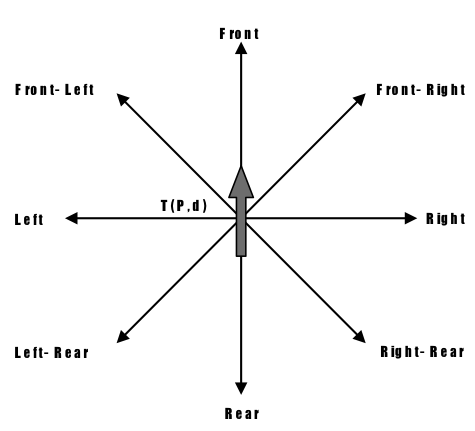
\includegraphics[width=0.33\textwidth, height=5cm]{2.RelatedWorks/fig2-b.png} \label{fig:img2-b} }
	\subfloat[]{ 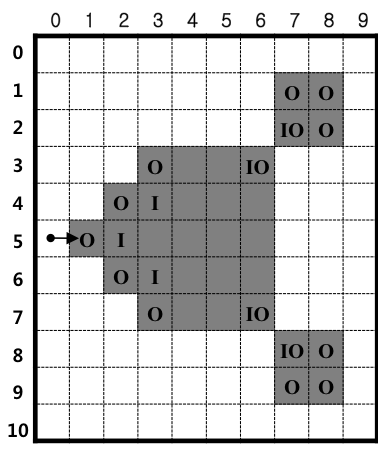
\includegraphics[width=0.31\textwidth, height=5cm]{2.RelatedWorks/fig2-c.png} \label{fig:img2-c} }
	 
	\caption{Directions and types of contour pixels. \protect\subref{fig:img2-a} Absolute direction $d$ \protect\subref{fig:img2-b} Relative direction $r$ \protect\subref{fig:img2-c} Types of contour pixels}
	\label{fig:image2}
\end{figure}


\subsubsection{Simple-boundary Follower}

% SBF is also known as Papert's turtle algorithm \cite{Das1990Bivariate} and as square tracing algorithm\cite{Toussaint????Grids}, and it is the simplest contour tracing algorithm. Initially, the location of tracer $S$ is saved, and the tracer moves leftward or rightward; if the pixel tracer is located on a contour pixel, the tracer moves leftward, otherwise it moves rightward. The procedure is as given below.

The simple-boundary follower (SBF) is also known as Papert's turtle algorithm \JHMEMO{[4]} and as a square-tracing algorithm \JHMEMO{[7]}, and it is the simplest contour-tracing algorithm. Initially, the location of tracer $S$ is saved, and the tracer moves in a left or right direction. If the pixel tracer is located on a contour pixel, the tracer moves left; otherwise, it moves right. The procedure is as given below.

\begin{algorithm}
	\caption{Algorithm of Simple Boundary Follower}\label{alg:sbf}
	\begin{algorithmic}[1]
	\Procedure{SBF}{}
	\State $\textit{T(P,d)} \gets \textit{S(P,d)}$
	\Do
	\If {$\textit{P}$ = black}
	\State $\textit{T(P,d)} \gets \textit{T(P}_{Left},\textit{d}_{Left} )  $
	\Else
	\State $\textit{T(P,d)} \gets \textit{T(P}_{Right},\textit{d}_{Right})$
	\EndIf
	\doWhile {$ \textit{T(P,d)}  \neq \textit{S(P,d)}$}
	\EndProcedure
	\end{algorithmic}
\end{algorithm}

\subsubsection{Modified Simple-boundary Follower}

% SBF cannot trace an inner-outer corner pixel that is located at the left-rear. MSBF \cite{Gose1996Pattern} was invented to trace these pixels. If the tracer is adjacent to the left-rear inner-outer corner, this condition implies that its left-rear pixel is black (object) and the left and rear pixels are white (background); the tracer will move to the left-rear pixel and its direction is then changed toward the rear direction. After the movement, the tracer goes directly to the left pixel to avoid an infinite loop. Figure \ref{fig:image3} shows examples of the SBF and MSBF paths for a left-rear direction inner-outer corner. In the case of the SBF, if the tracer is on pixel $A$ with direction $N$, it misses pixel $B$. On the contrary, the MSBF can detour pixel $B$.

SBF cannot trace an inner-outer corner pixel that is located at the left rear, and the modified SBF (MSBF) \JHMEMO{[3]} was developed to trace these pixels. If the tracer is adjacent to the left-rear inner-outer corner, this condition implies that its left-rear pixel is black (object), and the left and rear pixels are white (background); the tracer will move to the left-rear pixel, and its direction is then changed toward the rear direction. After the movement, the tracer goes directly to the left pixel to avoid an infinite loop. Figure \ref{fig:image3} shows examples of the SBF and MSBF paths for a left-rear direction inner-outer corner. In the case of the SBF, if the tracer is on pixel $A$ with direction $N$, it misses pixel $B$. On the contrary, the MSBF can detour pixel $B$.

%%% Image 3
\begin{figure}[htbp]
	\centering
	\subfloat[]{ 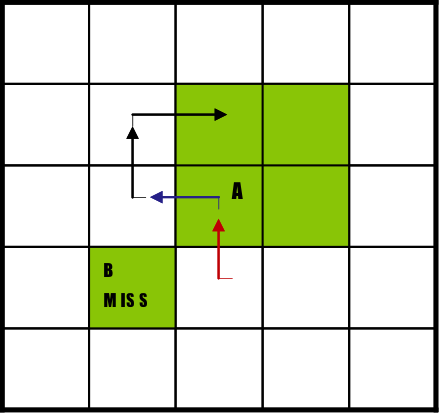
\includegraphics[width=0.3\textwidth]{2.RelatedWorks/fig3-a.png} \label{fig:img3-a} }
	\subfloat[]{ 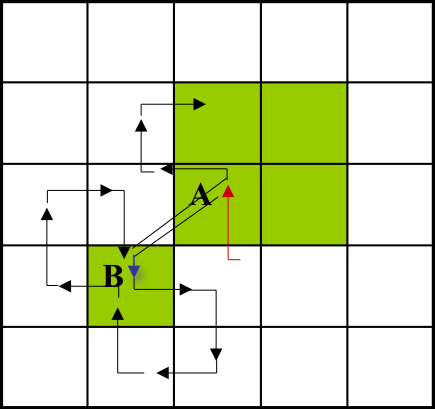
\includegraphics[width=0.3\textwidth]{2.RelatedWorks/fig3-b.png} \label{fig:img3-b} }
	 
	\caption{Detour of inner-outer corner at left-rear pixel (modified version of \cite{Gose1996Pattern}). \protect\subref{fig:img3-a} SBF \protect\subref{fig:img3-b} MSBF}
	\label{fig:image3}
\end{figure}

\subsubsection{Improved Simple-boundary Follower}

The SBF and MSBF require movement operations for both contour and background pixels; therefore, they waste time during movement on the background pixel and they cannot trace the inner corner pixel in front of the tracer \cite{Cheong2006Improved,Toussaint????Grids}. Hence, the ISBF \cite{Cheong2006Improved} is proposed based on our previous research for overcoming these limitations. The ISBF has six cases for following contour pixels based on the local patterns of the contour pixels. The modified version of \cite{Cheong2006Advanced} is as follows: 

The SBF and MSBF require movement operations for both contour and background pixels; therefore, time is wasted during movement on the background pixel, and they cannot trace the inner-corner pixel in front of the tracer [6,7]. Hence, we propose an improved SBF (ISBF) [6] that is based on our previous research aimed at overcoming these limitations. The ISBF has six cases for following-contour pixels based on the local patterns of the contour pixels. The modified version of Ref. [10] is as follows: 

\begin{algorithm}
	\caption{Algorithm of Improved Simple Boundary Follower}\label{alg:isbf}
	\begin{algorithmic}[1]
	\Procedure{ISBF}{}
	\State $\textit{T(P,d)} \gets \textit{S(P,d)}$, where \textit{P} is on black
	\Do
	\If {$\textit{P}_{Left}$ = black}
		\LineComment{Case \ref{fig:img4-a}: Left neighbor}
		\State $\textit{T(P,d)} \gets \textit{T(P}_{Left},\textit{d}_{Left} )  $
	\Else
		\If {$\textit{P}_{Left-Rear}$ = black and $\textit{P}_{Rear}$ = white}
			\LineComment{Case \ref{fig:img4-b}: Inner-outer corner at left-rear}
			\State $\textit{T(P,d)} \gets \textit{T(P}_{Left-Rear},\textit{d}_{Rear} )  $
		\Else
			\If {$\textit{P}_{Front-Left}$ = black}
				\If {$\textit{P}_{Front}$ = black}
					\LineComment{Case \ref{fig:img4-d}: Inner corer at front}
					\State $\textit{T(P,d)} \gets \textit{T(P}_{Front},\textit{d} )  $
					\State $\textit{T(P,d)} \gets \textit{T(P}_{Left}, \textit{d})$
				\Else
					\LineComment{Case \ref{fig:img4-c}: Inner-outer corner at front-left}
					\State $\textit{T(P,d)} \gets \textit{T(P}_{Front-Left},\textit{d} )  $
				\EndIf
			\ElsIf {$\textit{P}_{Front}$ = black}
				\LineComment{Case \ref{fig:img4-e}: Front neighbor}
				\State $\textit{T(P,d)} \gets \textit{T(P}_{Front},\textit{d}_{Right} )  $
			\Else
				\LineComment{Case \ref{fig:img4-f}: Outer corner}
				\State $\textit{T(P,d)} \gets \textit{T(P},\textit{d}_{Rear} )  $
			\EndIf
		\EndIf
	\EndIf
	\doWhile {$ \textit{T(P,d)}  \neq \textit{S(P,d)}$}
	\EndProcedure
	\end{algorithmic}
\end{algorithm}

% Figure \ref{fig:image4} represents the tracing path of the ISBF based on the local contour patterns. While the SBF cannot trace in cases \ref{fig:img4-b} and \ref{fig:img4-d}, and the MSBF cannot follow in case \ref{fig:img4-d}, the ISBF successfully traces in all the cases. In the figure, the way point (dotted line) is subjected to a detection operation for determining whether it is black or white without employing a movement operation.

Figure \ref{fig:image4} represents the tracing path of the ISBF based on the local contour patterns. While the SBF cannot trace in cases \ref{fig:img4-b} and \ref{fig:img4-d}, and the MSBF cannot follow in case \ref{fig:img4-d}, the ISBF successfully traces in all the cases. In the figure, the waypoint (dotted line) is subjected to a detection operation to determine whether it is black or white without employing a movement operation.

%%% Image 4
\begin{figure}[htbp]
	\centering
	\subfloat[]{ 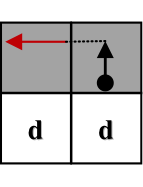
\includegraphics[height=2cm]{2.RelatedWorks/fig4-a.png} \label{fig:img4-a} }
	\subfloat[]{ 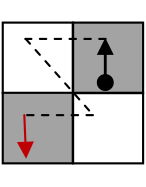
\includegraphics[height=2cm]{2.RelatedWorks/fig4-b.png} \label{fig:img4-b} }
	\subfloat[]{ 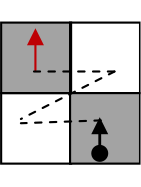
\includegraphics[height=2cm]{2.RelatedWorks/fig4-c.png} \label{fig:img4-c} }
	\subfloat[]{ 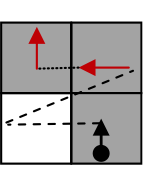
\includegraphics[height=2cm]{2.RelatedWorks/fig4-d.png} \label{fig:img4-d} }
	\subfloat[]{ 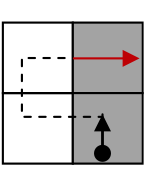
\includegraphics[height=2cm]{2.RelatedWorks/fig4-e.png} \label{fig:img4-e} }
	\subfloat[]{ 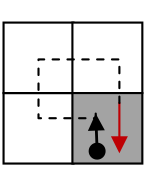
\includegraphics[height=2cm]{2.RelatedWorks/fig4-f.png} \label{fig:img4-f} }
	\subfloat{ 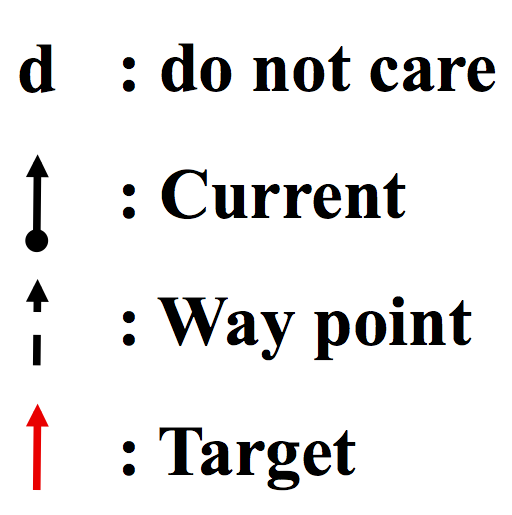
\includegraphics[height=2cm]{2.RelatedWorks/fig4-g.png} }
	 
	\caption{Contour cases of ISBF \cite{Cheong2006Advanced} \protect\subref{fig:img4-a} Left neighbor \protect\subref{fig:img4-b} Inner-outer corner at left-rear  \protect\subref{fig:img4-c} Inner-outer corner at front-left  \protect\subref{fig:img4-d} Inner corner at front \protect\subref{fig:img4-e} Front neighbor \protect\subref{fig:img4-f} Outer corner}
	\label{fig:image4}
\end{figure}

\subsubsection{Moore-Neighbor Tracing}
% MNT (see, figure \ref{fig:img5-a}) finds the next contour pixel using 8 connected chain codes using a clockwise sequence starting from the rear pixel of the tracer, i.e., the tracer first moves toward the rear ($T (P_{Rear}, d_{Rear}))$ and finds the next clockwise contour pixel such as the left-rear, left, font-left, front, front-right, right, and right-rear pixels \cite{Toussaint????Grids}. 
Moore-neighbor tracing (MNT) finds the next contour pixel using eight connected chain codes with a clockwise sequence starting from the rear pixel of the tracer, i.e., the tracer first moves toward the rear ($T (P_{Rear}, d_{Rear})$), and finds the next clockwise contour pixel such as the left-rear, left, font-left, front, front-right, right, and rear-right pixels \cite{Ghuneim2000Contour}\JHMEMO{HERE!!!} [7]. 

%%%%%%%%%%%%%%%%%%%%%% TO BE WRITTEN!!!!
%%%%%%%%%%%%%%%%%%%%%% TO BE WRITTEN!!!!
%%%%%%%%%%%%%%%%%%%%%% TO BE WRITTEN!!!!
% \subsubsection{Modified Moore-Neighbor Tracing}
% \JHMEMO{To be written}
%%%%%%%%%%%%%%%%%%%%%% TO BE WRITTEN!!!!
%%%%%%%%%%%%%%%%%%%%%% TO BE WRITTEN!!!!
%%%%%%%%%%%%%%%%%%%%%% TO BE WRITTEN!!!!

\subsubsection{Radial Sweep Algorithm}
% RSA \cite{Mirante1982Radial} is similar to MNT, but its tracer has no directional information. Therefore, it maintains two points, namely, previous pixel and current pixel for the initial tracing direction. Figure \ref{fig:img5-b} illustrates an example of a tracing path by using RSA from $P_i$ to $P_{i+2}$. In the figure, the direction vector from $P_i$ to $P_{i-1}$ is first generated, and then the tracer searches for the next contour pixel using the previous pixel $P_{i-1}$ for the clockwise direction of the vector.

The radial sweep algorithm (RSA) [8] is similar to MNT, but its tracer has no directional information. Therefore, it maintains two points, namely, the previous pixel and current pixel for the initial tracing direction. Figure \ref{fig:img5-b} illustrates an example of a tracing path obtained using RSA from $P_i$ to $P_{i+2}$. In the figure, the direction vector from $P_i$ to $P_{i-1}$ is first generated, and the tracer then searches for the next contour pixel using the previous pixel $P_{i-1}$ for the clockwise direction of the vector.

%%% Image 5
\begin{figure}[htbp]
	\centering
	\subfloat[]{ 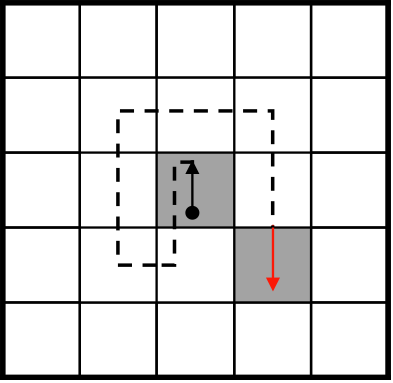
\includegraphics[width=0.3\textwidth]{2.RelatedWorks/fig5-a.png} \label{fig:img5-a} }
	\subfloat[]{ 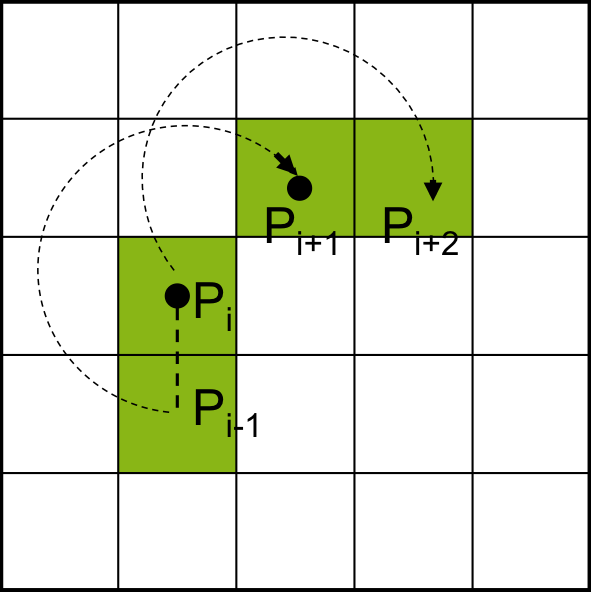
\includegraphics[width=0.3\textwidth]{2.RelatedWorks/fig5-b.png} \label{fig:img5-b} }
	\caption{Contour-following sequence of MNT and RSA \protect\subref{fig:img5-a} MNT \protect\subref{fig:img5-b} RSA}
	\label{fig:mnt_rsa}
\end{figure}

\subsubsection{Theo Pavlidis Algorithm}
% TPA \cite{Pavlidis2012Algorithms} considers only three adjacent pixels, e.g., front-left, front, and front-right for determining the next contour pixel. If all the three pixels are white, the tracer turns right. Figure \ref{fig:image6} describes its sequence. 
To determine the next contour pixel, the Theo Pavlidis algorithm (TPA) [9] considers only three adjacent pixels, e.g., front-left, front, and front-right. If all three pixels are white, the tracer turns right. Figure \ref{fig:image6} describes the sequence of this algorithm. 

%%% Image 6
\begin{figure}[htbp]
	\centering
	\subfloat[]{ 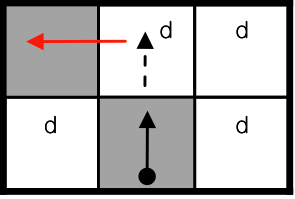
\includegraphics[width=0.25\textwidth]{2.RelatedWorks/fig6-a.png} \label{fig:img6-a} }
	\subfloat[]{ 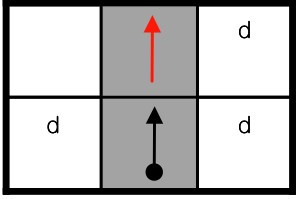
\includegraphics[width=0.25\textwidth]{2.RelatedWorks/fig6-b.png} \label{fig:img6-b} }
	\subfloat[]{ 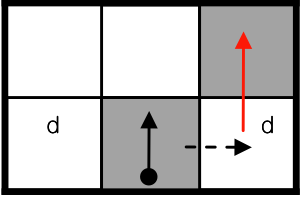
\includegraphics[width=0.25\textwidth]{2.RelatedWorks/fig6-c.png} \label{fig:img6-c} }
	\subfloat[]{ 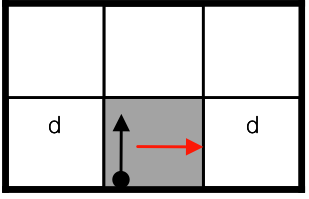
\includegraphics[width=0.25\textwidth]{2.RelatedWorks/fig6-d.png} \label{fig:img6-d} }
	 
	\caption{Contour-following sequence of TPA\cite{Cheong2006Advanced}. \protect\subref{fig:img6-a} Front-left contour \protect\subref{fig:img6-b} Front contour \protect\subref{fig:img6-c} Front-right contour \protect\subref{fig:img6-d} Rotation}
	\label{fig:image6}
\end{figure}

%%%%%%%%%%%%%%%%%%%%%%%%%%%%%
\subsection{Conventional Data Compression and Restoration}
% The RD code method \cite{Miyatake1997Contour} comprises two major techniques. One traces the contour on the basis of the hybrid method using vertex following with run data and generates the corresponding RD codes. The other generates compressed contour data that can be used to restore the contour on the basis of representative points and their corresponding RD codes. The representative points are selected from the vertices of contour pixels and they are feature points of the contour. Moreover, the RD code can represent 10 local contour patterns and their corresponding following paths. Therefore, saving the representative points and their corresponding RD codes rather than all the contour points can reduce the memory size used to store the contour data. Figure \ref{fig:img7-a} \cite{Miyatake1997Contour} gives an example of representative points. The representative points in the RD method are of four types, namely, two outer corner points and two inner corner points, as shown in figure \ref{fig:img7-b}. Although this technique can save data in small files; it does not consider the inner-outer corner pixel. 

The RD code method [11] comprises two major techniques. The first one traces the contour using a hybrid method that employs vertex following with run data, and it generates the corresponding RD codes. The other generates compressed contour data that can be used to restore the contour based on representative points and their corresponding RD codes. The representative points are selected from the vertices of contour pixels, and they are feature points of the contour. Moreover, the RD code can represent 10 local contour patterns and their corresponding following paths. Therefore, by saving the representative points and their corresponding RD codes instead of all the contour points, we can reduce the memory size used to store the contour data. Figure \ref{fig:img7-a} [11] gives an example of representative points. There are four types of representative points in the RD method, namely, two outer corner points and two inner corner points, as shown in Figure \ref{fig:img7-b}. Although this technique can save data in small files, it does not consider the inner-outer corner pixel. 

%%% Image 7
\begin{figure}[htbp]
	\centering
	\subfloat[]{ 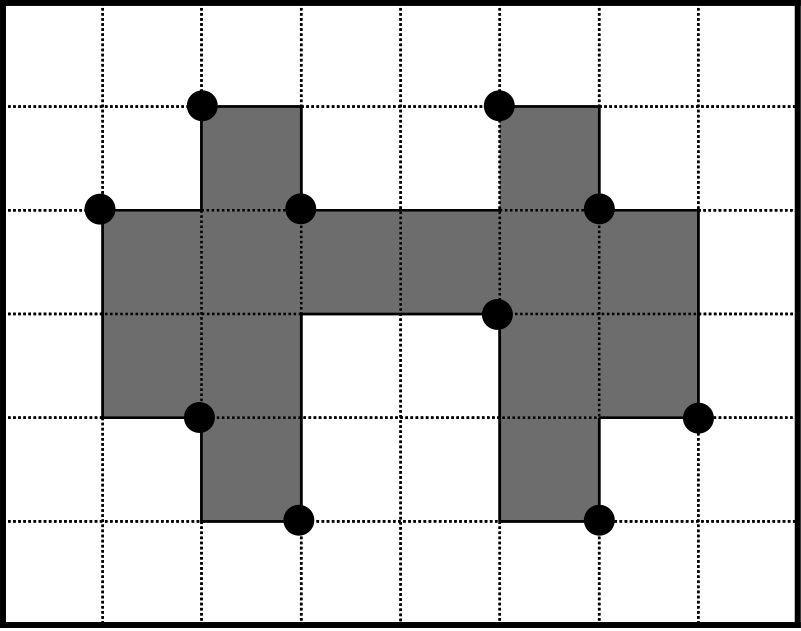
\includegraphics[height=4.5cm]{2.RelatedWorks/fig7-a.png} \label{fig:img7-a} }
	\subfloat[]{ 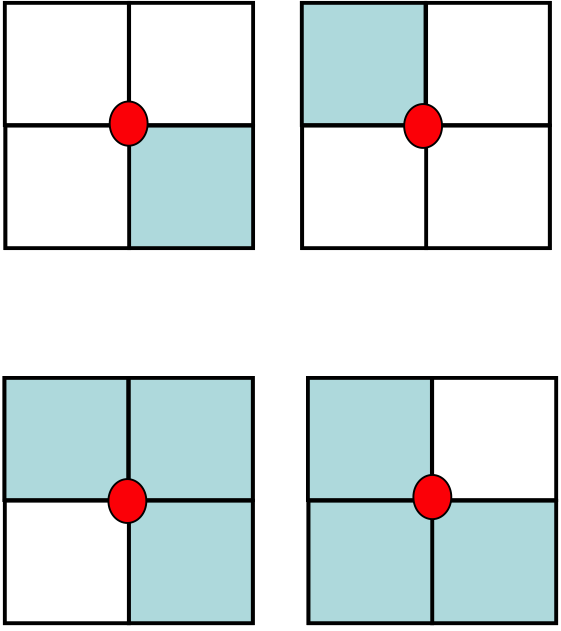
\includegraphics[height=4.5cm]{2.RelatedWorks/fig7-b.png} \label{fig:img7-b} }
	\caption{Representative points for data compression. \protect\subref{fig:img7-a} Representative points \cite{Miyatake1997Contour} \protect\subref{fig:img7-b} Cases of representative points}
	\label{fig:rdcode}
\end{figure}